\documentclass[11pt,a4paper]{article}

\usepackage[margin=1in]{geometry}
\usepackage{newtxtext,newtxmath}
\usepackage[T1]{fontenc}
\usepackage{microtype}
\usepackage{booktabs}
\usepackage{array}
\usepackage{graphicx}
\usepackage{xcolor}
\usepackage{enumitem}
\usepackage{caption}
\usepackage{amsmath}
\usepackage{placeins}
\usepackage{tikz}
\usetikzlibrary{arrows.meta,positioning,calc}
\usepackage{listings}
\usepackage{xspace}
\usepackage[numbers,sort&compress]{natbib}
\usepackage{url}
\usepackage{hyperref}
\usepackage{doi}

\hypersetup{
  colorlinks=true,
  linkcolor=black!70!blue,
  citecolor=black!70!blue,
  urlcolor=black!70!blue,
  pdftitle={CompilerSutraRun: A Reusable Execution and Validation Harness for Cross-API GPU Workloads},
  pdfauthor={Aditya Tiwari, Priya Pandey},
  pdfkeywords={GPU, orchestration, validation, reproducibility, Vulkan, OpenCL, HIP, OpenGL}
}

\captionsetup{font=small,labelfont=bf,skip=6pt}
\captionsetup[lstlisting]{font=small,labelfont=bf,skip=4pt}
\setlist[itemize]{nosep,leftmargin=1.2em}
\setlist[enumerate]{nosep,leftmargin=1.2em}

\lstdefinestyle{yaml}{
  basicstyle=\ttfamily\scriptsize,
  frame=single,
  rulecolor=\color{black!30},
  backgroundcolor=\color{black!3},
  breaklines=true,
  showstringspaces=false,
  columns=fullflexible,
  keepspaces=true,
  xleftmargin=0.4em,
  xrightmargin=0.4em
}

\newcommand{\csrun}{\texttt{csrun}\xspace}
\newcommand{\yes}{Y}
\newcommand{\no}{---}

\title{CompilerSutraRun: A Reusable Execution and Validation Harness\\
for Cross-API GPU Workloads}
\author{Aditya Tiwari \and Priya Pandey\\
{\small CompilerSutra}\\
{\small\texttt{\{aditya.tiwari, osc\}@compilersutra.com}}}
\date{}

\begin{document}
\maketitle

\begin{abstract}
Evaluating the same GPU operation across Vulkan, OpenGL, OpenCL, and HIP
requires more than backend-specific kernels: each path needs host scaffolding
for device selection, execution, correctness checking, and result collection.
When that scaffolding is rewritten per API, harness differences complicate
regression testing and make measurements hard to interpret.

We present \textbf{CompilerSutraRun} (\csrun), an open-source C++20 tool that
binds a single YAML workload contract to multiple GPU backends. The tool
separates workload configuration and result reporting from API-specific
compilation, resource management, dispatch, and synchronization. It provides
CPU-reference validation with an explicit numeric predicate, structured
\texttt{UNAVAILABLE} reporting for missing backends or devices, explicit
physical-device selection, and timing records that preserve their measurement
source. \csrun reuses existing toolchains (glslang, SPIR-V, vendor SDKs); it
does not introduce a new GPU IR or compiler.

We evaluate the implementation as a \emph{tool}: on a dual-GPU AMD Linux
workstation we execute vector addition ($N=1{,}048{,}576$ elements) through
Vulkan, OpenGL, OpenCL, and HIP on both a discrete Radeon~RX~9060~XT and an
integrated Raphael GPU. All eight paths pass CPU-reference validation and
report device-side timing (\texttt{gpu\_timestamp}). We do not claim that
these medians are cross-API performance rankings. Source, workloads, and
smoke artifacts are released under Apache-2.0 at
\url{https://github.com/compilersutra/CompilerSutraRun}.
\end{abstract}

\noindent\textbf{Keywords:}
GPU orchestration, correctness validation, reproducibility,
Vulkan, OpenCL, HIP, OpenGL, dual-GPU.

%======================================================================
\section{Introduction}
\label{sec:intro}

Modern GPU nodes often expose the same device through several
APIs---Vulkan~\cite{vulkan14}, OpenGL~\cite{opengl43},
OpenCL~\cite{opencl30}, and HIP~\cite{hipdocs} among them---each with its own
compilation model, memory rules, and timing facilities. Compiler, driver, and
performance engineers repeatedly need an answer to a narrow question:

\begin{quote}
\small\itshape
Does this operation still produce correct results on every API we claim to
support, and do our records preserve enough provenance to interpret the
measurements?
\end{quote}

In practice the answer is obtained by maintaining parallel host harnesses.
Timings are mixed without provenance (host wall-clock versus device
timestamps). Missing devices become silent skips that automated dashboards
misread as success.

Infrastructure projects such as LLVM~\cite{lattner2004llvm} and
MLIR~\cite{lattner2020mlir} reduce duplicated \emph{compiler} stacks.
Benchmark suites such as SHOC~\cite{danalis2010shoc} and
Rodinia~\cite{che2009rodinia} provide fixed kernel catalogs across CUDA and
OpenCL. Portable programming models such as SYCL~\cite{sycl2020} and
Kokkos~\cite{trott2022kokkos} raise abstraction above a single API, while
vendor profilers~\cite{nsight,rocprof} deepen measurement for one stack.
The remaining gap addressed here is a reusable \emph{execution and validation
harness} for user-defined workloads that spans multiple concrete APIs---including
modern Vulkan compute and HIP---with machine-readable availability and timing
provenance, without requiring the user to adopt a new programming model.

\paragraph{Contributions.}
This paper makes four contributions:
\begin{enumerate}
  \item A \textbf{workload contract} $W=(O,D,T,P,V)$ and a common backend
        interface that separates operation semantics from API-specific
        mechanisms (Section~\ref{sec:design}).
  \item A \textbf{validation and availability model}: CPU-reference checks,
        explicit validation states, and fail-closed \texttt{UNAVAILABLE}
        outcomes for stubs and missing devices (Section~\ref{sec:design}).
  \item A \textbf{measurement-provenance model}: per-run records that retain
        timing source, units, device identity, and environment metadata
        (Section~\ref{sec:design}).
  \item An open implementation and a dual-GPU functional study showing
        end-to-end execution and validation across four APIs
        (Section~\ref{sec:eval}).
\end{enumerate}

\noindent
\textbf{Scope.} A shared YAML description is \emph{not} shared GPU source:
kernels remain API-specific. \csrun is a tool for reproducible orchestration,
not a claim that different APIs have comparable absolute performance.
\FloatBarrier

%======================================================================
\section{Background and Related Work}
\label{sec:related}

We position \csrun against three classes of prior work.

\paragraph{Fixed benchmark suites.}
SHOC~\cite{danalis2010shoc} established scalable OpenCL/CUDA benchmarking for
heterogeneous nodes. Rodinia~\cite{che2009rodinia} targets scientific kernels
with OpenMP, OpenCL, and CUDA. These systems provide catalogs, not a portable
descriptor for arbitrary user workloads.

\paragraph{Peak and library tools.}
clpeak~\cite{clpeak2026} and mixbench~\cite{konstantinidis2015mixbench}
characterize device peaks and operational intensity. VkFFT~\cite{vkfft2021}
shows multi-API depth for one algorithm family. Vendor tools such as
Nsight~\cite{nsight} and rocprof~\cite{rocprof} provide rich counters within
one vendor stack.

\paragraph{Portable programming models.}
SYCL~\cite{sycl2020} and Kokkos~\cite{trott2022kokkos} aim at write-once
kernels across backends. \csrun is complementary and lower in the stack: it
orchestrates \emph{existing} API-specific kernels under a common host contract
rather than replacing those kernels with a new language or abstraction.

\begin{table}[htbp]
\centering
\small
\begin{tabular}{@{}lcccc@{}}
\toprule
System & User YAML & CPU-ref & Device index & Timing source \\
\midrule
SHOC~\cite{danalis2010shoc}     & \no & \no  & cluster MPI & suite-defined \\
Rodinia~\cite{che2009rodinia}   & \no & app  & \no         & app-defined \\
clpeak~\cite{clpeak2026}        & \no & \no  & flags       & peaks \\
mixbench~\cite{konstantinidis2015mixbench} & \no & \no & per binary & roofline \\
VkFFT~\cite{vkfft2021}          & \no & FFT  & build-time  & library \\
SYCL~/~Kokkos~\cite{sycl2020,trott2022kokkos} & \no & model & runtime & impl.-defined \\
\textbf{\csrun}                 & \yes & \yes & \yes$^\ast$ & labeled \\
\bottomrule
\end{tabular}
\caption{Related systems. ``User YAML'' means a portable descriptor for
user workloads (not a fixed catalog). ``CPU-ref'' means systematic
host-reference validation in the harness. ``Timing source'' means whether
result records identify how time was measured.
$^\ast$Vulkan/OpenCL/HIP via \texttt{--device-index}; OpenGL via
\texttt{DRI\_PRIME} (Section~\ref{sec:impl}).}
\label{tab:related}
\end{table}
\FloatBarrier

%======================================================================
\section{Design}
\label{sec:design}

\subsection{Workload contract}

A workload is
\[
W = (O,\, D,\, T,\, P,\, V),
\]
where $O$ is the operation and its mathematical semantics, $D$ the
input/output dimensions, $T$ the data-type specification, $P$ execution
parameters (warmup and measured iterations), and $V$ the validation policy.
Backend $B_i$ produces output $Y_i$ and measurement record $M_i$. Correctness
requires $Y_i$ to satisfy $V$ relative to a CPU reference; $M_i$ must state
what was measured and how.

For vector addition, $O$ is element-wise $c_i=a_i+b_i$,
$D$ sets $N=|a|=|b|=|c|$, $T$ is fp32, $P$ defaults to 10~warmup and
100~measured iterations, and $V$ uses the predicate below.
Listing~\ref{lst:yaml} shows the shipped descriptor.

\begin{lstlisting}[style=yaml,caption={Vector-add workload
(\texttt{examples/vector\_add/vector\_add.yaml}).},label={lst:yaml}]
name: vector_add
operation: vector_add
dimensions:
  count: 1048576          # N = 1,048,576 = 2^20
dtype: { input: fp32, output: fp32 }
execution: { warmup: 10, iterations: 100 }
validation: { enabled: true, tolerance: 1.0e-5 }
\end{lstlisting}

\subsection{Architecture}

Figure~\ref{fig:arch} separates a shared control plane from API adapters.
Vendor headers never enter common code. Stubs remain registered so missing
paths surface as \texttt{UNAVAILABLE} rather than omitted rows. Each backend
exposes \texttt{name()}, \texttt{available()}, and
\texttt{execute(workload, options)} so the CLI, validation path, and JSON
emitter stay API-agnostic.

\begin{figure}[htbp]
\centering
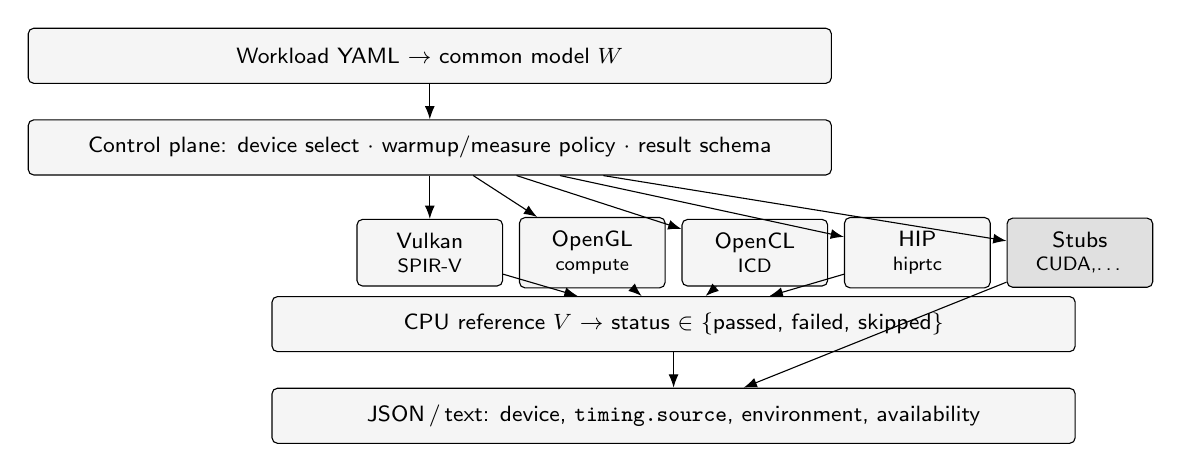
\begin{tikzpicture}[
  font=\sffamily\footnotesize,
  >=Latex,
  box/.style={draw, rounded corners=2pt, align=center, inner sep=5pt,
              minimum height=0.7cm, fill=black!4}
]
  \node[box, minimum width=10.2cm] (parse) {Workload YAML $\rightarrow$ common model $W$};
  \node[box, below=0.45cm of parse, minimum width=10.2cm] (ctrl)
    {Control plane: device select $\cdot$ warmup/measure policy $\cdot$ result schema};
  \node[box, below=0.55cm of ctrl, minimum width=1.85cm] (vk) {Vulkan\\[-1pt]\scriptsize SPIR-V};
  \node[box, right=0.2cm of vk, minimum width=1.85cm] (gl) {OpenGL\\[-1pt]\scriptsize compute};
  \node[box, right=0.2cm of gl, minimum width=1.85cm] (cl) {OpenCL\\[-1pt]\scriptsize ICD};
  \node[box, right=0.2cm of cl, minimum width=1.85cm] (hip) {HIP\\[-1pt]\scriptsize hiprtc};
  \node[box, right=0.2cm of hip, minimum width=1.85cm, fill=black!12] (stub)
    {Stubs\\[-1pt]\scriptsize CUDA,\ldots};
  \node[box, below=0.55cm of $(vk)!0.5!(hip)$, minimum width=10.2cm] (val)
    {CPU reference $V$ $\rightarrow$ status $\in$ \{passed, failed, skipped\}};
  \node[box, below=0.45cm of val, minimum width=10.2cm] (out)
    {JSON\,/\,text: device, \texttt{timing.source}, environment, availability};
  \draw[->] (parse) -- (ctrl);
  \draw[->] (ctrl) -- (vk);
  \draw[->] (ctrl) -- (gl);
  \draw[->] (ctrl) -- (cl);
  \draw[->] (ctrl) -- (hip);
  \draw[->] (ctrl) -- (stub);
  \draw[->] (vk) -- (val);
  \draw[->] (gl) -- (val);
  \draw[->] (cl) -- (val);
  \draw[->] (hip) -- (val);
  \draw[->] (stub) -- (out);
  \draw[->] (val) -- (out);
\end{tikzpicture}
\caption{CompilerSutraRun architecture. The shared plane owns parsing,
selection, validation policy, and the result schema. Adapters own
API-specific compile, buffers, dispatch, synchronization, and timers.
Grey stubs report \texttt{UNAVAILABLE}.}
\label{fig:arch}
\end{figure}

\subsection{Validation predicate}

For fp32 outputs, an element mismatches if and only if both absolute and
relative errors exceed their tolerances:
\begin{equation}
|a-b| > \epsilon_{\mathrm{abs}}
\;\wedge\;
\frac{|a-b|}{\max(|b|,10^{-12})} > \epsilon_{\mathrm{rel}}.
\label{eq:pred}
\end{equation}
The conjunction (rather than a max-of-thresholds rule) avoids failing large
magnitudes on tiny absolute noise while still catching large relative errors
on small values when both thresholds are exceeded. YAML \texttt{tolerance}
sets $\epsilon_{\mathrm{abs}}=\epsilon_{\mathrm{rel}}$. Disabling validation
yields status \texttt{skipped}, never \texttt{passed}. Unit tests cover
known-bad outputs, size mismatches, and skip-versus-pass behavior.

\subsection{Timing provenance}

We distinguish two measurement modes (Figure~\ref{fig:timing}):
\begin{itemize}
  \item \textbf{Mode~B (preferred):} device timers---Vulkan timestamps,
        OpenGL \texttt{GL\_TIME\_ELAPSED}, HIP events, or OpenCL profiling
        events---reported as \texttt{gpu\_timestamp}.
  \item \textbf{Mode~A (fallback):} host wall-clock around dispatch plus
        required synchronization, reported as \texttt{cpu\_wall}.
\end{itemize}
Host-to-device and device-to-host transfers lie \emph{outside} the timed
loop for vector add. JSON field \texttt{timing.source} records the mode.
Mixing Mode~A and Mode~B in a single ranking table is a methodology error.

\begin{figure}[htbp]
\centering
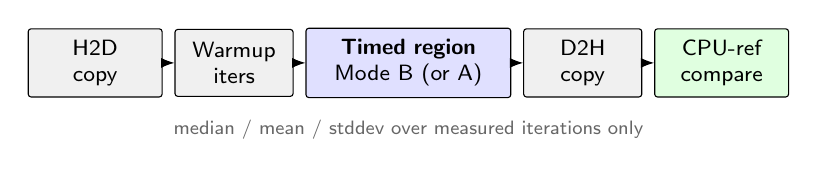
\begin{tikzpicture}[
  font=\sffamily\footnotesize,
  >=Latex,
  stage/.style={draw, align=center, minimum height=0.85cm, inner sep=4pt,
                rounded corners=1pt},
  note/.style={font=\sffamily\scriptsize, text=black!60}
]
  \node[stage, fill=black!6, minimum width=1.7cm] (h2d) {H2D\\copy};
  \node[stage, right=0.15cm of h2d, fill=black!6, minimum width=1.5cm] (warm) {Warmup\\iters};
  \node[stage, right=0.15cm of warm, fill=blue!12, minimum width=2.6cm] (timed)
    {\textbf{Timed region}\\Mode B (or A)};
  \node[stage, right=0.15cm of timed, fill=black!6, minimum width=1.5cm] (d2h) {D2H\\copy};
  \node[stage, right=0.15cm of d2h, fill=green!12, minimum width=1.7cm] (cmp) {CPU-ref\\compare};
  \draw[->] (h2d) -- (warm);
  \draw[->] (warm) -- (timed);
  \draw[->] (timed) -- (d2h);
  \draw[->] (d2h) -- (cmp);
  \node[note, below=0.15cm of timed]
    {median / mean / stddev over measured iterations only};
\end{tikzpicture}
\caption{Vector-add measurement boundary. Reported medians cover only the
timed region (dispatch + sync as defined by the backend timer). Transfers
and validation are recorded separately when available.}
\label{fig:timing}
\end{figure}

%======================================================================
\section{Implementation}
\label{sec:impl}

\csrun is implemented in C++20 (CMake~$\geq$~3.20, Ninja). Optional
dependencies enable backends at configure time; absent SDKs become stubs.
Kernels for vector add are authored per API
(\texttt{.comp}, \texttt{.cl}, \texttt{.hip}, GLSL). A Vulkan-oriented
matmul example exists but is \emph{not} counted as multi-API evaluation.

\begin{table}[t]
\centering
\small
\begin{tabular}{@{}p{2.2cm}p{2.2cm}p{7.8cm}@{}}
\toprule
Backend & Status & Notes \\
\midrule
Vulkan  & supported & SPIR-V via glslang; \texttt{--device-index} \\
OpenGL  & supported & EGL headless compute; discrete GPU via
                      \texttt{DRI\_PRIME=1} (not \texttt{--device-index}) \\
OpenCL  & supported & ICD; profiling queue for Mode~B \\
HIP     & supported & hiprtc; \texttt{--device-index} \\
Others  & stub & CUDA, D3D12, Metal, WebGPU, GLES, CPU backend:
                 registered as \texttt{UNAVAILABLE} \\
\bottomrule
\end{tabular}
\caption{Backend status. ``Supported'' means vector-add execute + validate
paths exist in the evaluated tree. Stubs are not execution backends.}
\label{tab:backends}
\end{table}
\FloatBarrier

\paragraph{Supported versus stub.}
A backend is \emph{supported} only if it can enumerate devices (when present),
execute the vector-add contract, and emit validation plus timing provenance.
Stubs remain visible in \texttt{--list-backends} so CI can distinguish
``not built'' from ``built but failed.''

%======================================================================
\section{Evaluation}
\label{sec:eval}

\subsection{Experimental setup}

\begin{table}[t]
\centering
\small
\begin{tabular}{@{}p{3.2cm}p{9.0cm}@{}}
\toprule
Item & Configuration \\
\midrule
CPU & AMD Ryzen~7 9700X \\
Discrete GPU & Radeon RX~9060~XT (Navi~44 / GFX1200), PCI \texttt{03:00.0} \\
Integrated GPU & Radeon Graphics (Raphael / GFX1036), PCI \texttt{15:00.0} \\
OS / kernel & Linux 7.0.0-34-generic (Ubuntu 24.04-based host) \\
Vulkan & Mesa RADV (ICD forced to \texttt{radeon\_icd.json}) \\
OpenGL & Mesa radeonsi \\
OpenCL / HIP & ROCm ICD / HIP runtime as enumerated on host \\
Workload & vector\_add, $N=1{,}048{,}576$ fp32, warmup~10, iters~100 \\
Artifact & \texttt{experiments/raw/revalidate-20261020/} \\
\bottomrule
\end{tabular}
\caption{Machine and software configuration for the functional study.}
\label{tab:machine}
\end{table}

We treat this study as a \textbf{functional smoke evaluation}: it demonstrates
that the harness can select devices, execute, validate, and label timing
sources. It is not a multi-batch statistical performance comparison.

\subsection{Results}

Table~\ref{tab:smoke} reports one archived batch. Every row uses Mode~B
(\texttt{gpu\_timestamp}). The reported standard deviation is the
\emph{within-batch} dispersion over the 100 measured iterations of that
single run---not the variability across independently restarted experiments.

\begin{table}[t]
\centering
\small
\begin{tabular}{@{}llrrr@{}}
\toprule
Backend & Device & Val. & Median (ms) & Std.\ (ms) \\
\midrule
Vulkan & RX~9060~XT & passed & 0.383 & 0.010 \\
Vulkan & Raphael    & passed & 0.400 & 0.013 \\
HIP    & RX~9060~XT & passed & 0.052 & 0.038 \\
HIP    & Raphael    & passed & 0.397 & 0.012 \\
OpenCL & gfx1200    & passed & 0.020 & 0.035 \\
OpenCL & gfx1036    & passed & 0.382 & 0.024 \\
OpenGL & RX~9060~XT & passed & 0.017 & 0.001 \\
OpenGL & Raphael    & passed & 0.380 & 0.017 \\
\bottomrule
\end{tabular}
\caption{Functional smoke ($N=1{,}048{,}576$, Mode~B;
artifact \texttt{revalidate-20261020}).
Std.\ is within-run dispersion ($n{=}100$), not multi-run IQR.
Medians are not a cross-API ranking.}
\label{tab:smoke}
\end{table}

\paragraph{Findings.}
\begin{enumerate}
  \item The same workload contract executed on both GPUs across four APIs
        with CPU-reference status \texttt{passed} in all eight cells.
  \item Explicit device selection is required on dual-GPU hosts:
        \texttt{--device-index} for Vulkan/OpenCL/HIP, and
        \texttt{DRI\_PRIME=1} for OpenGL discrete (OpenGL exposes a single
        EGL context and does not yet implement \texttt{--device-index}).
  \item OpenCL reports Mode~B through event profiling when a profiling
        queue is available; Mode~A remains the documented fallback.
  \item Without forcing the Mesa RADV ICD, the host can enumerate only
        llvmpipe---illustrating why fail-closed availability matters.
\end{enumerate}

\paragraph{What this study does not claim.}
We do not claim harness-LOC reduction ratios, multi-workload correctness
coverage, or statistically stable cross-API timings. Those require
additional artifact experiments beyond this tool paper's scope.

%======================================================================
\section{Limitations and Threats to Validity}
\label{sec:limits}

\paragraph{External validity.}
Results come from a single AMD workstation. CUDA, Metal, D3D12, and WebGPU
remain stubs; we do not imply NVIDIA or Apple support from registration alone.

\paragraph{Construct validity.}
Only vector add is evaluated end-to-end across four APIs. A Vulkan matmul
example exists but is not a multi-API result. Within-batch standard deviation
must not be read as experiment-level confidence intervals.

\paragraph{Internal validity.}
Sub-millisecond medians are sensitive to timer placement and driver state.
OpenGL device selection uses an environment mechanism distinct from
\texttt{--device-index}, which can confound naive cross-backend scripts.
Power samples, when present, are opportunistic metadata and are not primary
evidence.

%======================================================================
\section{Conclusion}
\label{sec:conc}

CompilerSutraRun provides a reusable contract for describing, executing, and
validating GPU workloads across Vulkan, OpenGL, OpenCL, and HIP, with explicit
device selection and labeled timing provenance. On a dual-GPU AMD host, the
same vector-add workload completes and validates on all four APIs for both
devices. We release the implementation and smoke artifacts under Apache-2.0
so others can inspect what is portable, what is validated, what is measured,
and what remains unsupported.

\section*{Availability}
Source repository:
\url{https://github.com/compilersutra/CompilerSutraRun}
(release tag \texttt{v0.1.0-paper}).
Smoke JSON under \path{experiments/raw/revalidate-20261020/}.
Timing and validation contracts:
\path{docs/timing-model.md}, \path{docs/validation.md}.

\bibliographystyle{plainnat}
\bibliography{references}

\end{document}
